\chapterimage{Water1.png} % Chapter heading image

\chapter{Water Laboratory Procedures}

\begin{enumerate}
\item Sampling\\
\begin{itemize}
\item Valid testing starts with an adequate and representative sampling. A sample is either a grab or a composite. A grab sample, as the name indicates, is a specific volume collected at one site at one time. These samples indicate the quality of water at that time and at that site. Grab samples are taken for bacteriological and disinfection residual tests. A composite sample is a mixture of a number of portions taken at the specific intervals. This reduces the number of tests. Each portion can be proportionate to the flow or volume. For each test operators should follow the prescribed sampling size, collecting, and preserving procedure given in the Standard Methods for the Examination of Water and Waste Water. Testing must be done as soon as possible and not later than the specified holding time.

\item One objective of surveillance is to assess the quality of water supplied by the supply agency and of that at the point of use, so that samples of both should be taken. Any significant difference between the two has important implications for remedial strategies. Samples must be taken from locations that are representative of the water source, treatment plant, storage facilities, distribution network, points at which water is delivered to the consumer, and points of use.

\item The most important tests used in water quality surveillance or quality control in small communities are those for microbiological quality (by the measurement of indicator bacteria) and turbidity, and for free chlorine residual and pH where chlorination is used. These tests should be carried out whenever a sample is taken, regardless of how many other physical or chemical variables are to be measured.

\item Although recommendations vary, the time between sample collection and analysis should, in general, not exceed 6 hours, and 24 hours is considered the absolute maximum. It is assumed that the samples are immediately placed in a lightproof insulated box containing melting ice or ice-packs with water to ensure rapid cooling. If ice is not available, the transportation time must not exceed 2 hours. It is imperative that samples are kept in the dark and that cooling is rapid. If these conditions are not met, the samples should be discarded. When water that contains or may contain even traces of chlorine is sampled, the chlorine must be inactivated. If it is not, microbes may be killed during transit and an erroneous result will be obtained. The bottles in which the samples are placed should therefore contain sodium thiosulfate to neutralize any chlorine present. The box used to carry samples should be cleaned and disinfected after each use to avoid contaminating the surfaces of the bottles and the sampler's hands.

\item In general, the time between sampling and analysis should be kept to a minimum. Storage in glass or polyethylene bottles at a low temperature in the dark is recommended. Sample bottles must be clean but need not be sterile. Special preservatives may be required for some analytes. Residual chlorine, pH, and turbidity should be tested immediately after sampling as they will change during storage and transport.
\end{itemize}





\item Bacteriological Analysis\\
\begin{itemize}
\item The principal risk associated with water in small-community supplies is that of infectious disease related to fecal contamination. Hense the microbiological examination of drinking water emphasizes assessment of the hygienic quality of the supply. This requires the isolation and enumeration of organisms that indicate the presence of fecal contamination. In certain circumstances, the same indicator organisms may also be used to assess the efficiency of drinking water treatment plants, which is an importat element of quality control.
 
\item Coliform organisms have long been recognized as a suitable microbial indicator of drinking water quality, largely because they are easy to detect and enumerate in water. The term "coliform organisms" refers to gram-negative, rod-shaped bacteria capable of growth in the presence of bile salts or other surface-active agents with similar growth- inhibiting properties and able to ferment lactose at 35-37°C with the production of acid gas, and aldehyde within 24-48 hours. Coliform bacteria should not be detectable in treated water supplies and, if found, suggest inadequate treatment, post-treatment contamination, or excessive nutrients. The coliform test can therefore be used as an indicator both of treatment efficiency and of the integrity of the distribution system.
Although coliform organisms may not always be directly related to the presence of fecal contamination or pathogens in drinking water, the coliform test is still useful for monitoring the microbial quality of treated piped water supplies.
\end{itemize}



\item Physicochemical Analysis Chlorine Residual\\
\begin{itemize}
\item The disinfection of drinking water supplies constitutes an important barrier against waterborne dieseases. Although various disinfectants may be used, chlorine in one form or another is the principal disinfecting agent employed. Chlorine has a number of advantages as a disinfectant, including its relative cheapness, efficacy, and ease of measurement, both in laboratories and in the field. An important additional advantage over some other disinfectants is that chlorine leaves a disinfectant residual that assists in preventing recontamination during distribution, transport, and household storage of water. The absence of a chlorine residual in the distribution system may, in certain circumstances, indicate the possibility of post-treatment contamination.

\item Three types of chlorine residual may be measured: free chlorine (the most reactive species); combined chlorine (less reactive but more persistent species formed by the reaction of free chlorine species with organic material and ammonia); and total chlorine (the sum of the free and combined chlorine residuals). Free chlorine is unstable in aqueous solution, and the chlorine content of water samples may decrease rapidly, particularly at warm temperatures. Exposure to strong light or agitation will accelerate the rate of loss of free chlorine. Water samples should therefore be analysed for free chlorine immediately on sampling and not stored for later testing.
\end{itemize}



\item pH
\begin{itemize}
\item It is important to measure pH at the same time as chlorine residual since the efficacy of disinfection with chlorine is highly pH-dependent; where the pH exceeds 8.0, disinfection is less effective. To check that the pH is in the optimal range for disinfection with chlorine (less than 8.0), simple tests may be conducted in the field using comparators such as that used for chlorine residual. With some chlorine comparators, it is possible to measure pH and chlorine residual simultaneously.

\item Alternatively, portable pH electrodes and meters are available. If these are used in the laboratory, they must be calibrated against fresh pH standards at least daily; for field use, they should be calibrated immediately before each test. Results may be inaccurate if the water has a low buffering capacity.
\end{itemize}



\item Turbidity
\begin{itemize}
\item Turbidity is a measure of the degree to which the water loses its transparency due to the presence of suspended particulates. The more total suspended solids in the water, the murkier it seems and the higher the turbidity. Turbidity is considered a good measure of the quality of water. Turbidity is important because it affects both the acceptability of water to consumers, and the selection and efficiency of treatment processes, particularly the efficiency of disinfection with chlorine since it exerts a chlorine demand and protects microorganisms and may also stimulate the growth of bacteria. In all processes in which disinfection is used, the turbidity must always be low - preferably below 1 NTU. It is recommended that, for water to be disinfected, the turbidity should be consistently less than 5 NTU. Turbidity may change during sample transit and storage, and should therefore be measured on site at the time of sampling.

\item Turbidity is the murkiness in the water caused by colloidal (1 to 100 nanometer particles) and other suspended particles, such as clay, sand, silt, organic matter of plant and animal origin, planktons, and other microscopic organisms. Turbidity particles can be waterborne pathogens or particles harboring them. The lower the turbidity, the less is the amount of the particulate matter. It means there is less probability of the presence of waterborne pathogens, and the water is safer. Therefore, turbidity is one of the primary standards for the drinking water. The finished water turbidity is tested at least every four hours.

\item Turbidity is measured as the amount of scattered light by the suspended particles in the sample. Turbidity of the finished water should be equal to or less than 0.3 nephalometric turbidity unit (NTU) in 95 percent of the samples/month.
\end{itemize}






\item Aesthetic Parameters
 \begin{itemize}
\item Aesthetic parameters are those detectable by the senses, namely turbidity, color, taste and odor. They are important in monitoring community water supplies because they may cause the water supply to be rejected and alternative, possibly poorer-quality, sources to be adopted, and they are simple and inexpensive to monitor qualitatively in the field.
\end{itemize}

\item Color
\begin{itemize}
\item Color in drinking water may be due to the presence of colored organic matter, e.g. humic substances, metals such as iron and manganese, or highly colored industrial wastes. Drinking water should be colorless. For the purposes of surveillance of community water supplies, it is useful simply to note the presence or absence of observable color at the time of sampling. Changes in the color of water and the appearance of new colors serve as indicators that further investigation is needed.
\end{itemize}



\item Tastes and Odors
\begin{itemize}
\item Odors in water are caused mainly by the presence of organic substances. Some odors are indicative of increased biological activity, others may result from industrial pollution. Sanitary inspections shoudl always include the investigation of possible or existing sources of odor, and attempts should always be made to correct an odor problem. Taste problems, which are sometimes grouped with odor problems, usually account for the largest single category of consumer complaints. Generally, the taste buds detect the inorganic compounds of metals such as magnesium, calcium, sodium, copper, iron, and zinc.

\item Testing for taste and odor is important because of aesthetic value. The majority of water quality complaints are of this type. Most of the organic and some inorganic chemicals cause tastes and odors. These chemicals come from the decaying organic matter, runoffs, industrial wastes, and municipal sewage discharges. Geosmin and methyl- isobarneol (MIB) are the serious odor-causing chemicals; they are produced by bacteria, particularly actinomycetes, while decomposing dead organic matter at the bottom of the water bodies. Even a very low concentration of these chemicals can cause earthy-musty odors. The odors are common in spring and fall due to the turn over of the lakes and reservoirs. 
\item In the groundwater, the tastes and odors can be due to iron, manganese, and hydrogen sulfide (H2S).
These are general classes of odors:
\begin{itemize}
\item Aromatic (spicy)
\item Balsamic (flowery) 
\item Chemical 
\item Disagreeable
\item Earthy
\item Musty
\item Grassy
\item Vegetable
\end{itemize}
 
\item These are called the reference odor in the water samples.
\end{itemize}


\section{Density}\index{Density}
\begin{itemize}
\item Density is defined as the weight of a substance per a unit of its volume. For example, pounds per cubic foot or pounds per gallon.

\item Here are a few key facts about density:
\begin{itemize}

\item Density is measured in units of lb/ft3, lb/gal, or mg/L. Density of water = 62.4 lb/ft3 = 8.34 lb/gal.
\item Density of concrete = 130 lb/ft3. Density of alum (liquid @ 60°F) = 1.33
\item Density of hydrogen peroxide (35%) = 1.132
\end{itemize}
\end{itemize}

\section{Specific Gravity}\index{Specific Gravity}
\begin{itemize}
\item Specific gravity is a relationship of the liquid to water. A liquid that is heavier than water will have a specific gravity greater than one. If you know the weight per gallon of the liquid you can find the specific gravity of the material by dividing the weight per gallon by the weight of one gallon of water.

\item Here are a few key facts about specific gravity:
\begin{itemize}
\item Specific gravity has no units. Specific gravity of water = 1.0 Specific gravity of concrete = 2.08
\item Specific gravity of alum (liquid @ 60°F) = 1.33 Specific gravity of hydrogen peroxide (35%) = 1.132
\end{itemize}


\item Any substance with a density greater than that of water will have a specific gravity greater than 1.0. Any substance with a density less than that of water will have a specific gravity less than 1.0. The density and specific gravity of a substance indicates whether it will sink or float in water. If its density is greater than that of water (1.0), it will sink; if less, it will float.
\end{itemize}

A liquid chemical is determined to weigh 9.17 lb/gal. What is the specific gravity of the chemical? Also, specify if the chemical will sink or float in the water?
 

 


This particular chemical will sink because its specific gravity is 1.1 and water's specific gravity is 1.0. Remember that above it states if its specific gravity is greater than that of water (1.0) it will sink.

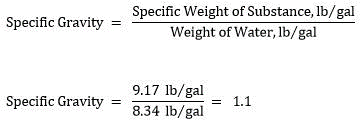
\includegraphics[scale=1]{SpecificGravityProblem1}

\item Review\\
\begin{itemize}
\item A number of lab tests are needed daily, quarterly, semiannually, annually, and at other specified intervals to monitor the water quality before, during, and after the treatment. A sample is either a grab or a composite. A grab sample, as the name indicates, is a specific volume collected at one site at one time. These samples indicate the quality of water at that time and at that site. Grab samples are taken for bacteriological and disinfection residual tests. A composite sample is a mixture of a number of portions taken at the specific intervals. This reduces the number of tests. Each portion can be proportionate to the flow or volume.

\item Various regularly performed common tests by the operating staff are for tastes and odor, turbidity, jar test, pH, alkalinity, hardness, disinfection residual, coliform bacteria, and the heterotrophic plate count. All other tests are run either by highly trained chemists and microbiologists of the lab or by certified contract laboratories.
\end{itemize}